%% Requires compilation with XeLaTeX or LuaLaTeX
\documentclass[10pt,xcolor={table,dvipsnames}]{beamer}
\usetheme{UVic}

\usepackage{booktabs}
\usepackage{amsmath}
\usepackage{amssymb}
\usepackage{tikz}
\usetikzlibrary{shapes.geometric, arrows.meta, positioning, fit, backgrounds}

% Reduce gap between header and frame title
\addtobeamertemplate{frametitle}{\vspace*{-2.2em}}{}

\title[PhD Committee Review]{PhD Committee Review}
\subtitle{Learning Automata Framework for Adaptive Kelp Forest Monitoring in British Columbia Coastal Waters}
\author{Ekaba Bisong}
\institute{Department of Computer Science\\University of Victoria\\[0.5em]Supervisor: Dr. Neil Ernst}
\date{January 28, 2026}

\begin{document}

% Slide 1: Title
\begin{frame}
  \titlepage
\end{frame}

% ============================================================================
\section{Introduction}
% ============================================================================

% Slide 2: Motivation (merged from Kelp Ecosystems + Monitoring Challenge)
\begin{frame}{Motivation}

\textbf{Why Kelp Matters:}
\begin{itemize}
  \item Among Earth's most productive ecosystems
  \item Critical habitat, carbon sequestration, coastal protection
  \item Deep cultural significance for BC First Nations
\end{itemize}

\vspace{0.3em}
\textbf{The Problem:}
\begin{itemize}
  \item BC kelp declining. Some regions $>$70\% loss (Starko 2024)
  \item Causes vary: thermal stress (south), urchin barrens (north)
\end{itemize}

\vspace{0.3em}
\textbf{Monitoring Challenge:}
\begin{itemize}
  \item No single algorithm works across all conditions
  \item Labels are sparse and arrive with delays
  \item Need adaptive system that learns from limited feedback
\end{itemize}

\end{frame}

% Slide 3: Problem Statement
\begin{frame}{Problem Statement}

\textbf{Core Challenge:}

How can we develop an automated kelp monitoring system that:

\begin{enumerate}
  \item Adapts to heterogeneous environmental conditions across BC's coastline?

  \item Learns effectively with limited labeled training data?

  \item Handles sparse and delayed ground-truth validation?

  \item Fuses multi-source data (10m imagery to 5km oceanographic) with missing data?

  \item Integrates Traditional Ecological Knowledge respectfully?
\end{enumerate}

\vspace{0.3em}
\textbf{Proposed Solution:} A Learning Automata framework for adaptive heuristic selection

\end{frame}

% ============================================================================
\section{Research Questions}
% ============================================================================

% Slide 4: Research Questions
\begin{frame}{Research Questions}

\begin{itemize}
  \item \textbf{RQ1 (Adaptation):} How effectively can an LA framework adapt to new regions with limited labeled examples?

  \vspace{0.3em}
  \item \textbf{RQ2 (Heterogeneity):} Can context-aware heuristic selection improve accuracy across heterogeneous coastal environments?

  \vspace{0.3em}
  \item \textbf{RQ3 (Sparse Labels):} How can delayed and sparse ground-truth feedback be incorporated into learning?

  \vspace{0.3em}
  \item \textbf{RQ4 (Data Fusion):} How can heterogeneous data sources (10m--5km) be fused for context-aware adaptation despite resolution mismatches and missing data?

  \vspace{0.3em}
  \item \textbf{RQ5 (TEK Integration):} What protocols enable respectful integration of Traditional Ecological Knowledge?
\end{itemize}

\end{frame}

% ============================================================================
\section{Background}
% ============================================================================

% Slide 5: Learning Automata (merged from 3 slides)
\begin{frame}{Learning Automata: Adaptive Decision-Making}

\begin{columns}[T]
\begin{column}{0.55\textwidth}
\textbf{Core Concept:}
\begin{itemize}
  \item Agent selects action with probability $p_i$
  \item Environment returns reward/penalty
  \item Update probabilities based on feedback
\end{itemize}

\vspace{0.3em}
\textbf{L$_{\text{R-I}}$ Scheme:}
\begin{itemize}
  \item On reward: increase $p_i$
  \item On penalty: no change (inaction)
  \item Converges to optimal action
\end{itemize}
\end{column}

\begin{column}{0.42\textwidth}
\textbf{Why LA for Kelp?}
\begin{itemize}
  \item Handles sparse, noisy feedback
  \item No retraining needed
  \item Proven $\epsilon$-optimal convergence
  \item Adapts to non-stationary environments (seasonal + regime shifts)
\end{itemize}
\end{column}
\end{columns}

\end{frame}

% ============================================================================
\section{Proposed Methodology}
% ============================================================================

% Slide 6: Framework Architecture Diagram (from proposal)
\begin{frame}{Framework Architecture}

\centering
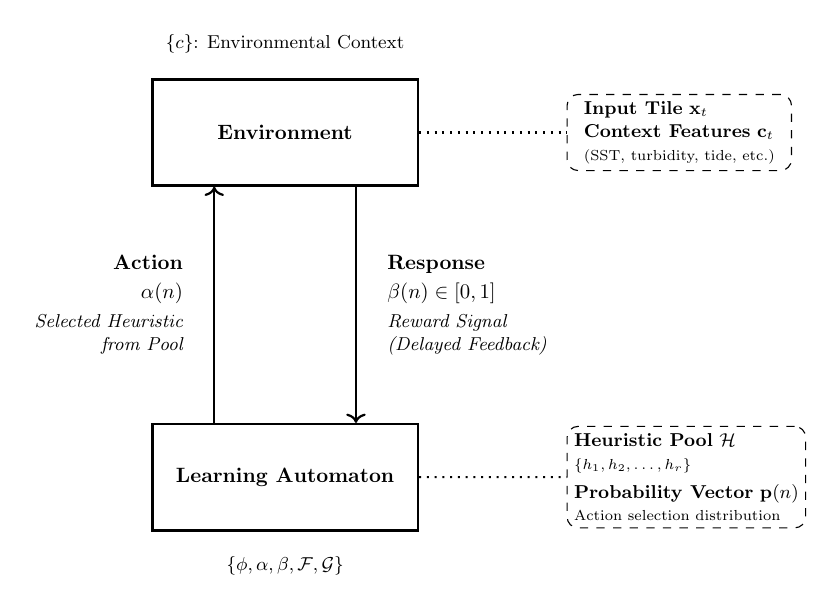
\begin{tikzpicture}[
    scale=0.75, transform shape,
    % Styles
    mainbox/.style={
        rectangle,
        draw=black,
        line width=1pt,
        minimum width=4.5cm,
        minimum height=1.8cm,
        align=center,
        font=\bfseries
    },
    label/.style={
        font=\small\itshape
    },
    tuple/.style={
        font=\small
    },
    arrow/.style={
        ->,
        thick,
        line width=0.8pt
    }
]

% Environment Box
\node[mainbox] (env) at (0, 0) {Environment};

% Environment set notation above
\node[tuple, above=0.3cm of env] {$\{c\}$: Environmental Context};

% Automaton Box
\node[mainbox, below=4cm of env] (auto) {Learning Automaton};

% Automaton tuple below
\node[tuple, below=0.3cm of auto] {$\{\phi, \alpha, \beta, \mathcal{F}, \mathcal{G}\}$};

% Left arrow: Action (Automaton to Environment)
\draw[arrow] ([xshift=-1.2cm]auto.north) -- ([xshift=-1.2cm]env.south)
    node[midway, left=0.4cm, align=right] {
        \textbf{Action}\\[2pt]
        $\alpha(n)$\\[2pt]
        {\small\itshape Selected Heuristic}\\[-1pt]
        {\small\itshape from Pool}
    };

% Right arrow: Response/Reward (Environment to Automaton)
\draw[arrow] ([xshift=1.2cm]env.south) -- ([xshift=1.2cm]auto.north)
    node[midway, right=0.4cm, align=left] {
        \textbf{Response}\\[2pt]
        $\beta(n) \in [0,1]$\\[2pt]
        {\small\itshape Reward Signal}\\[-1pt]
        {\small\itshape (Delayed Feedback)}
    };

% Component annotations on the right side
\node[draw, dashed, rounded corners, minimum width=3.8cm, minimum height=1.2cm,
      right=2.5cm of env, align=left, font=\small] (env_detail) {
    \textbf{Input Tile} $\mathbf{x}_t$\\
    \textbf{Context Features} $\mathbf{c}_t$\\
    {\scriptsize (SST, turbidity, tide, etc.)}
};
\draw[dotted, thick] (env.east) -- (env_detail.west);

\node[draw, dashed, rounded corners, minimum width=3.8cm, minimum height=1.6cm,
      right=2.5cm of auto, align=left, font=\small] (auto_detail) {
    \textbf{Heuristic Pool} $\mathcal{H}$\\
    {\scriptsize $\{h_1, h_2, \ldots, h_r\}$}\\[3pt]
    \textbf{Probability Vector} $\mathbf{p}(n)$\\
    {\scriptsize Action selection distribution}
};
\draw[dotted, thick] (auto.east) -- (auto_detail.west);

\end{tikzpicture}

\end{frame}

% Slide 7: Framework Components (merged from 6 slides)
\begin{frame}{Framework Components}

\textbf{Component 1: Global Policy Learning}
\begin{itemize}
  \item L$_{\text{R-I}}$ updates maintain probability distribution over heuristics
  \item Heuristic pool: Spectral indices (NDVI, FAI) $\rightarrow$ ML (RF, SVM) $\rightarrow$ DL (U-Net, ViT)
\end{itemize}

\vspace{0.3em}
\textbf{Component 2: Context-Aware Local Adaptation}
\begin{itemize}
  \item Context features: spectral, spatial, temporal, environmental, geographic
  \item Memory bank with k-NN retrieval for local probability estimation
  \item Blending: $\mathbf{p}_{\text{final}} = \alpha \cdot \mathbf{p}_{\text{global}} + (1-\alpha) \cdot \mathbf{p}_{\text{local}}$
\end{itemize}

\vspace{0.3em}
\textbf{Component 3: Sparse Label Handling}
\begin{itemize}
  \item Prediction buffer stores outputs until labels arrive
  \item Temporal decay: $\gamma^{(t_{\text{now}} - t_{\text{pred}})}$ downweights stale feedback
  \item Enables learning from asynchronous validation
\end{itemize}

\end{frame}

% ============================================================================
\section{Experimental Design}
% ============================================================================

% Slide 8: Experimental Design (merged dataset + protocols + ablations)
\begin{frame}{Experimental Design}

\textbf{Dataset:}
\begin{itemize}
  \item Sentinel-2 imagery (10m resolution), BC coastline, 2017--2024
  \item Ground truth: Kelp surveys, drone validation, TEK observations
  \item Environmental: Sea surface temperature (SST), turbidity, tide data
\end{itemize}

\vspace{0.3em}
\textbf{Evaluation Protocols:}
\begin{itemize}
  \item \textbf{Temporal:} Train Year 1 $\rightarrow$ Test Years 2--3
  \item \textbf{Spatial:} Leave-one-region-out cross-validation
  \item \textbf{Sparse Labels:} Vary delay distributions (days to months)
\end{itemize}

\vspace{0.3em}
\textbf{Ablations:} Global-only vs. context-aware; with/without temporal decay; heuristic tier analysis

\vspace{0.3em}
\textbf{Metrics:} F1-score, Precision, Recall, IoU

\end{frame}

% ============================================================================
\section{Contributions}
% ============================================================================

% Slide 9: Contributions
\begin{frame}{Expected Contributions}

\textbf{Scientific \& Methodological:}
\begin{itemize}
  \item Novel LA framework for environmental monitoring
  \item Context-aware heuristic selection methodology
  \item Sparse label learning with temporal decay
  \item \textbf{Multi-source data fusion framework} for coastal monitoring
  \item TEK integration protocols respecting data sovereignty
\end{itemize}

\vspace{0.4em}
\textbf{Practical Impact:}
\begin{itemize}
  \item Scalable kelp monitoring for BC's 26,000+ km coastline
  \item Framework transferable to other ecosystems (seagrass, coral)
\end{itemize}

\vspace{0.4em}
\textbf{Publications:} 5 papers targeting RQ1--RQ5

\end{frame}

% Slide 11: Summary
\begin{frame}{Summary}

\begin{itemize}
  \item \textbf{Problem:} Adaptive kelp monitoring with limited labels and heterogeneous conditions

  \vspace{0.3em}
  \item \textbf{Solution:} Learning Automata framework with three components
  \begin{itemize}
    \item Global policy learning
    \item Context-aware local adaptation (enabled by multi-source data fusion)
    \item Sparse label handling
  \end{itemize}

  \vspace{0.3em}
  \item \textbf{Validation:} Five research questions with rigorous experimental design

  \vspace{0.3em}
  \item \textbf{Timeline:} October 2027 completion with five publications

  \vspace{0.3em}
  \item \textbf{Impact:} Scalable monitoring supporting kelp conservation in BC
\end{itemize}

\end{frame}

% Slide 12: Questions
\begin{frame}{}

\vspace{2em}
\centering
{\Huge Thank You}

\vspace{1.5em}
{\Large Questions?}

\vspace{2em}
\normalsize
Ekaba Bisong\\
ebisong@uvic.ca

\end{frame}

% ============================================================================
% BACKUP SLIDES
% ============================================================================

% Backup: Consolidated Timeline
\begin{frame}{Backup: Timeline}

\begin{columns}[T]
\begin{column}{0.48\textwidth}
\textbf{2026: Foundation}
\begin{itemize}
  \item Jan: Proposal defense
  \item May (M1): Dataset + baselines
  \item Aug: Paper 1 (RQ4 Data Fusion)
  \item Oct (M2): Core framework
  \item Nov: Paper 2 (RQ1)
\end{itemize}
\end{column}

\begin{column}{0.48\textwidth}
\textbf{2027: Completion}
\begin{itemize}
  \item Jan (M3): Temporal experiments
  \item Feb: Paper 3 (RQ2)
  \item Mar--Apr (M4-5): Spatial + sparse
  \item Apr: Paper 4 (RQ3)
  \item May--Jun (M6): TEK + Paper 5
  \item Aug (M7): Thesis draft
  \item Oct (M8): Defense
\end{itemize}
\end{column}
\end{columns}

\vspace{0.5em}
\centering
\textbf{Target:} 5 publications, October 2027 defense

\end{frame}

% Backup: LA Mathematical Details
\begin{frame}{Backup: L$_{\text{R-I}}$ Update Equations}

\textbf{Linear Reward-Inaction (L$_{\text{R-I}}$):}

On reward ($\beta = 0$) for action $\alpha_i$:
\begin{align}
p_i(n+1) &= p_i(n) + \lambda(1 - p_i(n)) \\
p_j(n+1) &= (1-\lambda)p_j(n), \quad j \neq i
\end{align}

On penalty ($\beta = 1$): No update (inaction)

\vspace{0.5em}
\textbf{Properties:}
\begin{itemize}
  \item $\lambda \in (0,1)$: Learning rate
  \item $\epsilon$-optimal in all stationary environments
  \item Robust to noisy feedback
\end{itemize}

\end{frame}

% Backup: Heuristic Pool Details
\begin{frame}{Backup: Heuristic Pool}

\textbf{Three-Tier Architecture:}

\begin{itemize}
  \item \textbf{Tier 1: Spectral Indices}
  \begin{itemize}
    \item NDVI, FAI, NDWI, Kelp Index
  \end{itemize}

  \item \textbf{Tier 2: Classical Machine Learning}
  \begin{itemize}
    \item Random Forest, SVM, XGBoost, Logistic Regression
  \end{itemize}

  \item \textbf{Tier 3: Deep Learning}
  \begin{itemize}
    \item U-Net, DeepLabV3+, ResNet, Vision Transformer
  \end{itemize}
\end{itemize}

\end{frame}

% Backup: RQ Validation Details
\begin{frame}{Backup: RQ Validation Strategy}

\textbf{RQ1 (Adaptation):} Vary labels 5\%--100\%; compare fixed heuristic, random, supervised CNN

\vspace{0.25em}
\textbf{RQ2 (Heterogeneity):} Stratify by turbidity, SST, geography; global vs. context-aware

\vspace{0.25em}
\textbf{RQ3 (Sparse Labels):} Simulate delays (days/weeks/months); measure convergence, stability

\vspace{0.25em}
\textbf{RQ4 (Data Fusion):} Ablate context features; compare alignment strategies; validate against in-situ data; test missing data robustness

\vspace{0.25em}
\textbf{RQ5 (TEK):} Site importance weights, temporal priors, elder validation; respect data sovereignty

\end{frame}

% Backup: Ablation Details
\begin{frame}{Backup: Ablation Studies}

\textbf{Component Ablations:}
\begin{itemize}
  \item Full framework vs. global-only (no context)
  \item Full framework vs. no temporal decay
  \item Full framework vs. immediate labels only
\end{itemize}

\vspace{0.5em}
\textbf{Hyperparameter Sensitivity:}
\begin{itemize}
  \item Learning rate $\lambda \in \{0.01, 0.05, 0.1, 0.2\}$
  \item Neighbors $k \in \{3, 5, 10, 20\}$
  \item Decay $\gamma \in \{0.9, 0.95, 0.99\}$
  \item Blending $\alpha \in \{0.3, 0.5, 0.7\}$
\end{itemize}

\end{frame}

% Backup: RQ2 Conceptual Model - Context-Aware Selection
\begin{frame}{Backup: RQ2 Context-Aware Heuristic Selection}

\centering
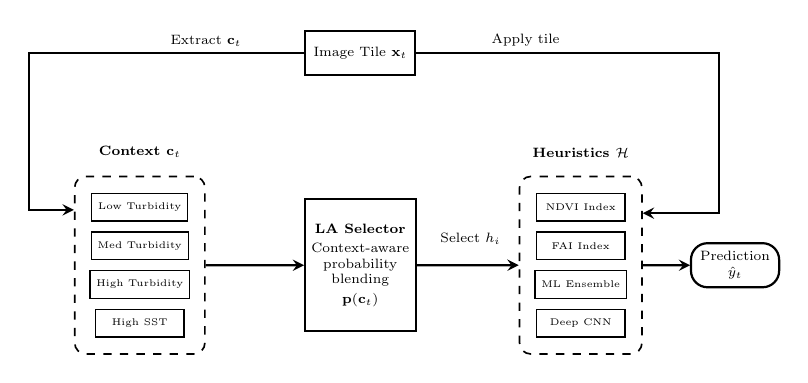
\begin{tikzpicture}[
    scale=0.7, transform shape,
    box/.style={rectangle, draw=black, line width=0.8pt, minimum width=2cm, minimum height=0.7cm, align=center, font=\scriptsize},
    smallbox/.style={rectangle, draw=black, line width=0.5pt, minimum width=1.6cm, minimum height=0.5cm, align=center, font=\tiny},
    inputbox/.style={rectangle, draw=black, line width=0.8pt, minimum width=2cm, minimum height=0.8cm, align=center, font=\scriptsize},
    outputbox/.style={rectangle, draw=black, line width=0.8pt, rounded corners=6pt, minimum width=1.6cm, minimum height=0.8cm, align=center, font=\scriptsize},
    groupbox/.style={rectangle, draw=black, line width=0.6pt, dashed, rounded corners=4pt},
    arrow/.style={->, thick, >=stealth}
]

% Input: Satellite Tile (center top)
\node[inputbox] (input) at (4, 3.5) {Image Tile $\mathbf{x}_t$};

% === Context Group (left side) ===
\node[smallbox] (cond1) at (0, 0.7) {Low Turbidity};
\node[smallbox] (cond2) at (0, 0) {Med Turbidity};
\node[smallbox] (cond3) at (0, -0.7) {High Turbidity};
\node[smallbox] (cond4) at (0, -1.4) {High SST};

% Dashed box around contexts
\node[groupbox, fit=(cond1)(cond4), inner sep=6pt] (contextbox) {};
\node[above=0.2cm of contextbox, font=\scriptsize\bfseries] {Context $\mathbf{c}_t$};

% === LA Selector (center) ===
\node[box, minimum height=2.4cm, minimum width=2cm] (la) at (4, -0.35) {
    \textbf{LA Selector}\\[2pt]
    Context-aware\\
    probability\\
    blending\\[2pt]
    $\mathbf{p}(\mathbf{c}_t)$
};

% === Heuristics Group (right side) ===
\node[smallbox] (h1) at (8, 0.7) {NDVI Index};
\node[smallbox] (h2) at (8, 0) {FAI Index};
\node[smallbox] (h3) at (8, -0.7) {ML Ensemble};
\node[smallbox] (h4) at (8, -1.4) {Deep CNN};

% Dashed box around heuristics
\node[groupbox, fit=(h1)(h4), inner sep=6pt] (heurbox) {};
\node[above=0.2cm of heurbox, font=\scriptsize\bfseries] {Heuristics $\mathcal{H}$};

% === Output: Prediction ===
\node[outputbox] (output) at (10.8, -0.35) {Prediction\\$\hat{y}_t$};

% === Arrows ===
\draw[arrow] (input.west) -- ++(-5,0) |- (contextbox.140);
\node[font=\scriptsize, above] at (1.2, 3.5) {Extract $\mathbf{c}_t$};

\draw[arrow] (input.east) -- ++(5.5,0) |- (heurbox.40);
\node[font=\scriptsize, above] at (7, 3.5) {Apply tile};

\draw[arrow] (contextbox.east) -- (la.west);
\draw[arrow] (la.east) -- (heurbox.west);
\node[font=\scriptsize, above] at (6, -0.1) {Select $h_i$};

\draw[arrow] (heurbox.east) -- (output.west);

\end{tikzpicture}

\end{frame}

% Backup: RQ3 Conceptual Model - Sparse Label Learning
\begin{frame}{Backup: RQ3 Sparse Label Learning}

\centering
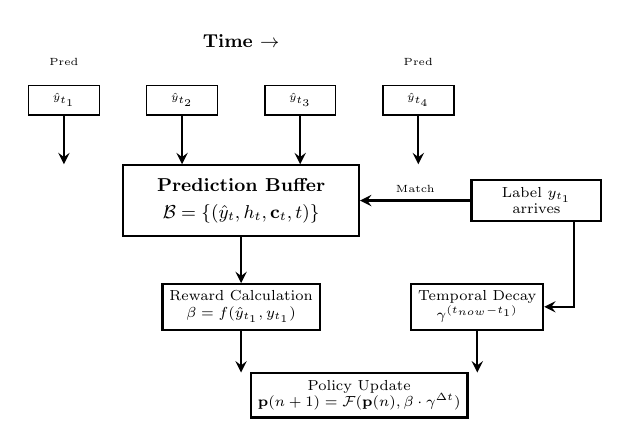
\begin{tikzpicture}[
    scale=0.75, transform shape,
    box/.style={rectangle, draw=black, line width=0.8pt, minimum width=2cm, minimum height=0.7cm, align=center, font=\scriptsize},
    timeline/.style={rectangle, draw=black, line width=0.6pt, minimum width=1.2cm, minimum height=0.5cm, align=center, font=\tiny},
    buffer/.style={rectangle, draw=black, line width=0.8pt, minimum width=4cm, minimum height=1.2cm, align=center, font=\small},
    arrow/.style={->, thick, >=stealth},
    dasharrow/.style={->, dashed, thick, >=stealth}
]

% Timeline at top
\node[font=\small\bfseries] at (0, 3) {Time $\rightarrow$};

% Prediction nodes
\node[timeline] (p1) at (-3, 2) {$\hat{y}_{t_1}$};
\node[timeline] (p2) at (-1, 2) {$\hat{y}_{t_2}$};
\node[timeline] (p3) at (1, 2) {$\hat{y}_{t_3}$};
\node[timeline] (p4) at (3, 2) {$\hat{y}_{t_4}$};

\node[above=0.2cm of p1, font=\tiny] {Pred};
\node[above=0.2cm of p4, font=\tiny] {Pred};

% Prediction Buffer
\node[buffer] (buf) at (0, 0.3) {
    \textbf{Prediction Buffer}\\[2pt]
    $\mathcal{B} = \{(\hat{y}_t, h_t, \mathbf{c}_t, t)\}$
};

% Arrows to buffer
\draw[arrow] (p1.south) -- (buf.north -| p1);
\draw[arrow] (p2.south) -- (buf.north -| p2);
\draw[arrow] (p3.south) -- (buf.north -| p3);
\draw[arrow] (p4.south) -- (buf.north -| p4);

% Delayed label arrival
\node[box, minimum width=2.2cm] (label) at (5, 0.3) {Label $y_{t_1}$\\arrives};

% Arrow from label to buffer lookup
\draw[arrow] (label.west) -- node[above, font=\tiny] {Match} (buf.east);

% Reward calculation
\node[box, minimum width=2.5cm] (reward) at (0, -1.5) {Reward Calculation\\$\beta = f(\hat{y}_{t_1}, y_{t_1})$};

\draw[arrow] (buf.south) -- (reward.north);

% Temporal decay
\node[box, minimum width=2.2cm] (decay) at (4, -1.5) {Temporal Decay\\$\gamma^{(t_{now} - t_1)}$};

\draw[arrow] (label.330) |- (decay.east);

% Policy update
\node[box, minimum width=3cm] (update) at (2, -3) {Policy Update\\$\mathbf{p}(n+1) = \mathcal{F}(\mathbf{p}(n), \beta \cdot \gamma^{\Delta t})$};

\draw[arrow] (reward.south) -- ++(0,-0.3) -| (update.north -| reward);
\draw[arrow] (decay.south) -- ++(0,-0.3) -| (update.north -| decay);

\end{tikzpicture}

\end{frame}

% Backup: RQ4 Conceptual Model - Multi-Source Data Fusion
\begin{frame}{Backup: RQ4 Multi-Source Data Fusion}

\centering
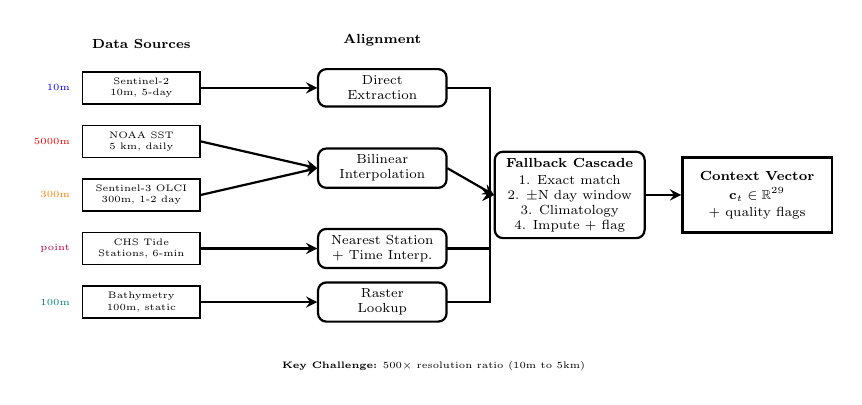
\begin{tikzpicture}[
    scale=0.68, transform shape,
    source/.style={rectangle, draw=black, line width=0.6pt, minimum width=2.2cm, minimum height=0.6cm, align=center, font=\tiny},
    process/.style={rectangle, draw=black, line width=0.8pt, rounded corners=3pt, minimum width=2.4cm, minimum height=0.7cm, align=center, font=\scriptsize},
    output/.style={rectangle, draw=black, line width=1pt, minimum width=2.8cm, minimum height=0.9cm, align=center, font=\scriptsize},
    arrow/.style={->, thick, >=stealth},
    dasharrow/.style={->, dashed, >=stealth}
]

% Data Sources (left column)
\node[source] (s2) at (0, 3) {Sentinel-2\\10m, 5-day};
\node[source] (sst) at (0, 2) {NOAA SST\\5 km, daily};
\node[source] (olci) at (0, 1) {Sentinel-3 OLCI\\300m, 1-2 day};
\node[source] (tide) at (0, 0) {CHS Tide\\Stations, 6-min};
\node[source] (bathy) at (0, -1) {Bathymetry\\100m, static};

\node[above=0.3cm of s2, font=\scriptsize\bfseries] {Data Sources};

% Resolution labels
\node[left=0.1cm of s2, font=\tiny, text=blue] {10m};
\node[left=0.1cm of sst, font=\tiny, text=red] {5000m};
\node[left=0.1cm of olci, font=\tiny, text=orange] {300m};
\node[left=0.1cm of tide, font=\tiny, text=purple] {point};
\node[left=0.1cm of bathy, font=\tiny, text=teal] {100m};

% Alignment Methods (middle column)
\node[process] (direct) at (4.5, 3) {Direct\\Extraction};
\node[process] (bilinear) at (4.5, 1.5) {Bilinear\\Interpolation};
\node[process] (nearest) at (4.5, 0) {Nearest Station\\+ Time Interp.};
\node[process] (lookup) at (4.5, -1) {Raster\\Lookup};

\node[above=0.3cm of direct, font=\scriptsize\bfseries] {Alignment};

% Missing Data Handling (right-middle)
\node[process, minimum width=2.8cm, minimum height=1.2cm] (fallback) at (8, 1) {
    \textbf{Fallback Cascade}\\[1pt]
    1. Exact match\\
    2. $\pm$N day window\\
    3. Climatology\\
    4. Impute + flag
};

% Output (right)
\node[output, minimum height=1.4cm] (context) at (11.5, 1) {
    \textbf{Context Vector}\\[2pt]
    $\mathbf{c}_t \in \mathbb{R}^{29}$\\[1pt]
    + quality flags
};

% Arrows from sources to alignment
\draw[arrow] (s2.east) -- (direct.west);
\draw[arrow] (sst.east) -- (bilinear.west);
\draw[arrow] (olci.east) -- (bilinear.west);
\draw[arrow] (tide.east) -- (nearest.west);
\draw[arrow] (bathy.east) -- (lookup.west);

% Arrows from alignment to fallback
\draw[arrow] (direct.east) -- ++(0.8,0) |- (fallback.west);
\draw[arrow] (bilinear.east) -- (fallback.west);
\draw[arrow] (nearest.east) -- ++(0.8,0) |- (fallback.west);
\draw[arrow] (lookup.east) -- ++(0.8,0) |- (fallback.west);

% Arrow from fallback to context
\draw[arrow] (fallback.east) -- (context.west);

% Annotation at bottom - positioned below all boxes
\node at (5.5, -2.2) [align=center, font=\tiny] {
    \textbf{Key Challenge:} 500$\times$ resolution ratio (10m to 5km)
};

\end{tikzpicture}

\vspace{0.3em}
\begin{columns}[T]
\begin{column}{0.48\textwidth}
\textbf{29 Context Features:}
\begin{itemize}\scriptsize
    \item 12 spectral (means, variances)
    \item 4 texture (GLCM)
    \item 3 temporal (DOY, gap, year)
    \item 5 environmental (SST, tide, Chl, Kd, solar)
    \item 5 geographic (lat, lon, depth, shore, fetch)
\end{itemize}
\end{column}
\begin{column}{0.48\textwidth}
\textbf{Quality Flags $q_i \in \{0,1,2,3\}$:}
\begin{itemize}\scriptsize
    \item 0 = Exact match
    \item 1 = Interpolated
    \item 2 = Climatology
    \item 3 = Imputed
\end{itemize}
\end{column}
\end{columns}

\end{frame}

\end{document}
